\chapter{Tests et analyse défauts fonctionnels ESD}
\label{chap:1}
\section{Contexte}

% What is an ESD, its key properties
An electrostatic discharge (ESD) is the result of the accumulation of electrostatic potential.
It is a very sudden current flow that propagates through metallic or non-metallic materials, electrical systems and sometimes even through the air.
It is a very short electrical event, involving large currents and extremely high voltages.
\gls{ESD} have durations in the range of a few hundred nanoseconds.
Currents can reach tens of amperes and voltage levels several thousand of volts.
The total discharge energy is small, somewhere near the milli-Joule (mJ).
The power on the other hand is extremely high because the waveforms are changing extremely rapidly.

% What generates an ESD
Objects can accumulate electrostatic potential by tribocharging or electrostatic induction.
In the case of tribocharging, electrons are transferred from one object the other when they are put into contact then separated.
One object becomes positively charged and the other negatively.
Which object gains electrons depends on the kind of material constituting each object.

% Electronic devices are exposed to ESD, in factories first
As detailed in the introduction, electrostatic discharges constitute a large threat for electronic devices.
Failures can occur during manufacturing and or normal operation.
The manipulation of parts by manufacturing machines involves repeated contact and separation.
Ultimately, triboelectrification and discharges happen and devices can get destroyed.
Several standards exist to guarantee that devices can survive this manufacturing step.

Parler HMM, MM, CDM
Tests for manufacturing env

% Electronic devices are exposed to ESD in the field
After manufacturing, failures can happen with the device in the field and exposed to its operating environment.
Manipulation by electrically-charged humans is a major source of danger for commercial products like cellphones and cameras.
The automotive environment is even harsher, with vehicles being a major source of electrostatic discharges.

% Hard-failure is one thing, soft-fail another
Integrated circuits are studied and protected against hard-failure since a few decades.
Despite this experience of the \gls{esd} community, it remains challenging to perfectly protect an electronic system against hard-failures.
Nowadays, a new class of failures appears.
Instead of studying permanent failures, devices are studied for temporary failures affecting their functionality.
These are called soft-failures or functional failures.
\gls{esd} can cause them to happen, with diverse consequences.
In less severe situations, functionnality of a chip is disturbed just for the duration of the ESD and recovers immediately without noticeable consequence.
The failure remains located inside the integrated circuit and does not impact the application above.
Sometimes, the discharge is harmful enough to cause a circuit to restart because the \gls{esd} disturbed some critial nets or parameters.
This is common when supply voltages go out of specification for instance.
Startups or power-on reset functions understands overvoltage or undervoltage as the signal for a regular power-up sequence.
The device can also perform restarts to try a recovery because proper operations cannot be guaranteed, due to unexpected values on some nets.
Most microcontrollers for instance monitor supply voltages of digital gates.
If the voltage is too low, the noise margins of the gates cannot be guaranteed and proper operations either.
At this point, the microcontroller restarts to try to recover.
Restarts are slow processes compared to the operation of a chip.
For critical applications, this delay is highly unwanted because it impacts human safety.
The availability of the chip that triggers airbags in a car is vital for instance.
In a more severe scenario, the system gets completely frozen or stuck into an unwanted state because of the \gls{esd}.
The only way to recover normal operation requires a user-intervention.
User intervention can take the form of turning the key to shut down and restart the vehicle's engine.
Finally, hard-failure can be seen as the next step immediately after the most severe soft-failure.
The device is in a non-recoverable state and must be replaced.
Hard-failures are not considered for functional robustness analysis.

\section{Méthodes de test ESD}

To reproduce disturbances in lab, multiple stress generators

% History of TLP
The transmission line pulsing generator is an extremely popular tool in the \gls{esd} field.
Over the years, it was employed in a variety of applications, from characterization of devices \cite{TLPforESDProtectionCz, TLPthroubleshooting}, investigation of failures \cite{tlp-application-1, tlp-application-2} and correlation of failure levels with other generators \cite{correlation-system-level-esd-tlp}.
It is a versatile tool, that was often modified to adress larger testing conditions \cite{tlp-power} or non-rectangular pulse waveforms \cite{tlp-based-hmm, my-publi-tlp-hmm}.
The technique was invented by T. Maloney and N. Nakamura \cite{TLP}.
It is in the process of standardization as part of ANSI/ESD STM 5.5.1-2016 \cite{tlp-standard} through the effort of the ESD Association (ESDA) \cite{esda}.
It was extensively studied during the PhD thesis of N. Monnereau \cite{phd-monnereau} and N. Lacrampe \cite{phd-lacrampe}.

% Concept
\gls{tlp} systems produce a short rectangular pulse, through the discharge of a coaxial cable (Fig. \ref{tlp_concept}).
The cable is initially charged with an high-voltage voltage supply through a high value resistor.
This keeps the current small and avoids oscillations on the cable.
When the voltage of the cable reaches the desired amplitude, a relay can be switched to trigger the discharge.
The coaxial cable has usually a characteristic impedance of 50\textOmega{} and a length of 5 metres, corresponding to a 50ns propagation delay.
The generated pulse is twice that delay.

\begin{figure}[!h]
  \centering
  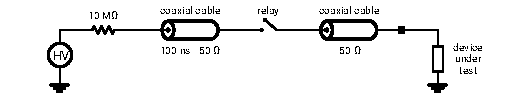
\includegraphics[width=\textwidth]{src/1/figures/tlp_concept.pdf}
  \caption{Minimal example of a \gls{tlp} system}
  \label{tlp_concept}
\end{figure}

% Characteristics of tlp systems
TLP systems constitute very well-controlled test generators.
The pulse is generated inside a shielded environment.
It is isolated from external radiated emissions and does not emit electromagnetic disturbances.
The characteristic impedance of 50\textOmega{} can be controlled up to the load, by using appropriate 50\textOmega{} cables and hardware.
Those properties result in clean and repeatable pulse waveforms without reflections.
The main features of the generated pulse are given in figure \ref{tlp_pulse}.

\begin{figure}[!h]
  \centering
  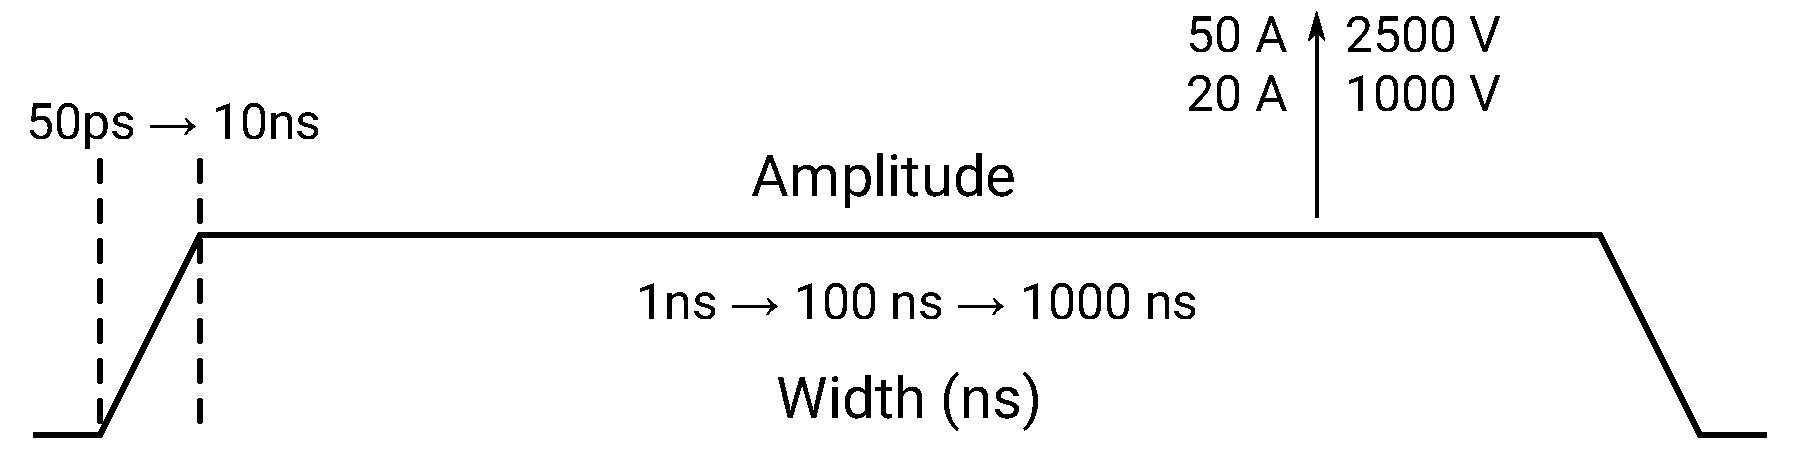
\includegraphics[width=\textwidth]{src/1/figures/tlp_pulse.pdf}
  \caption{Main characteristics of a \gls{tlp} pulse on a resistive load}
  \label{tlp_pulse}
\end{figure}


Pistolets de décharge ESD

% What is the goal of this test
IEC 61000-4-2 \cite{iec61000-4-2} and ISO 10605 \cite{iso10605} standards define a system-level test waveform and test generator to reproduce the discharge of a human body through an electronic device.
This test is used very extensively for qualification of products.
Fig. \ref{fig:picture-esd-gun} provides a picture of an \gls{esd} gun.
The gun is composed of a metallic discharge tip to inject the pulse.
The ground return is a long metallic ribbon a couple of meters long.
Depending on the test configuration, it is connected to the product ground or the earth.
Its shape impacts a lot recorded failure levels.
Historically, ESD gun were famous for lacking some reproducibility on test results \cite{hmm-uncertainty}.
They have largely improved since then although radiated emissions and shape of the ground return still remain a very large factor of variation and uncertainty \cite{gun-rf-uncertainty}.

% How is the pulse generated
The generation of the ESD pulse is done with a 330\textOmega resistor and 150 pF capacitor discharge network.
The RC network alone though does not suffice to reproduce the waveform.
Parasitic devices play an important part in shaping the waveform.
Fig. \ref{fig:esd-gun-model} provides a physically-based ESD Gun model that helps understand the impact of parasitic devices.
This model was originally written by Chiu \cite{phd-chiu} and is referenced in the PhD thesis of N. Monnereau \cite{phd-monnereau}.
It adds an R\textsubscript{g}L\textsubscript{g}C\textsubscript{g} network to model the ground return.
A parasitic capacitance C\textsubscript{i} and series inductance L\textsubscript{i} model imperfections in the direct injection path.

\begin{figure}[!h]
  \centering
  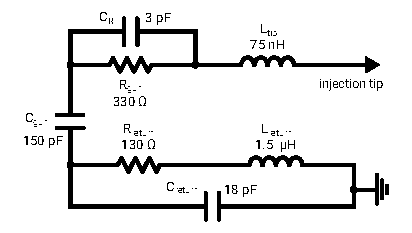
\includegraphics[width=0.3\textwidth]{src/1/figures/gun_model.pdf}
  \caption{ESD Gun model}
  \label{fig:esd-gun-model}
\end{figure}

% Explain the waveform
%TODO: Why 2 ohms ?
Fig. \ref{iec_pulse} presents the main properties of the generated stress.
The standard defines this waveform for a 2\textOmega{} load.
The pulse starts by a fast peak with a $1ns$ risetime.
It is followed by a slower slope of smaller amplitude but longer duration of about $200ns$.
Voltage levels can reach 15kV peak and 30A of current.

\begin{figure}[!h]
  \centering
  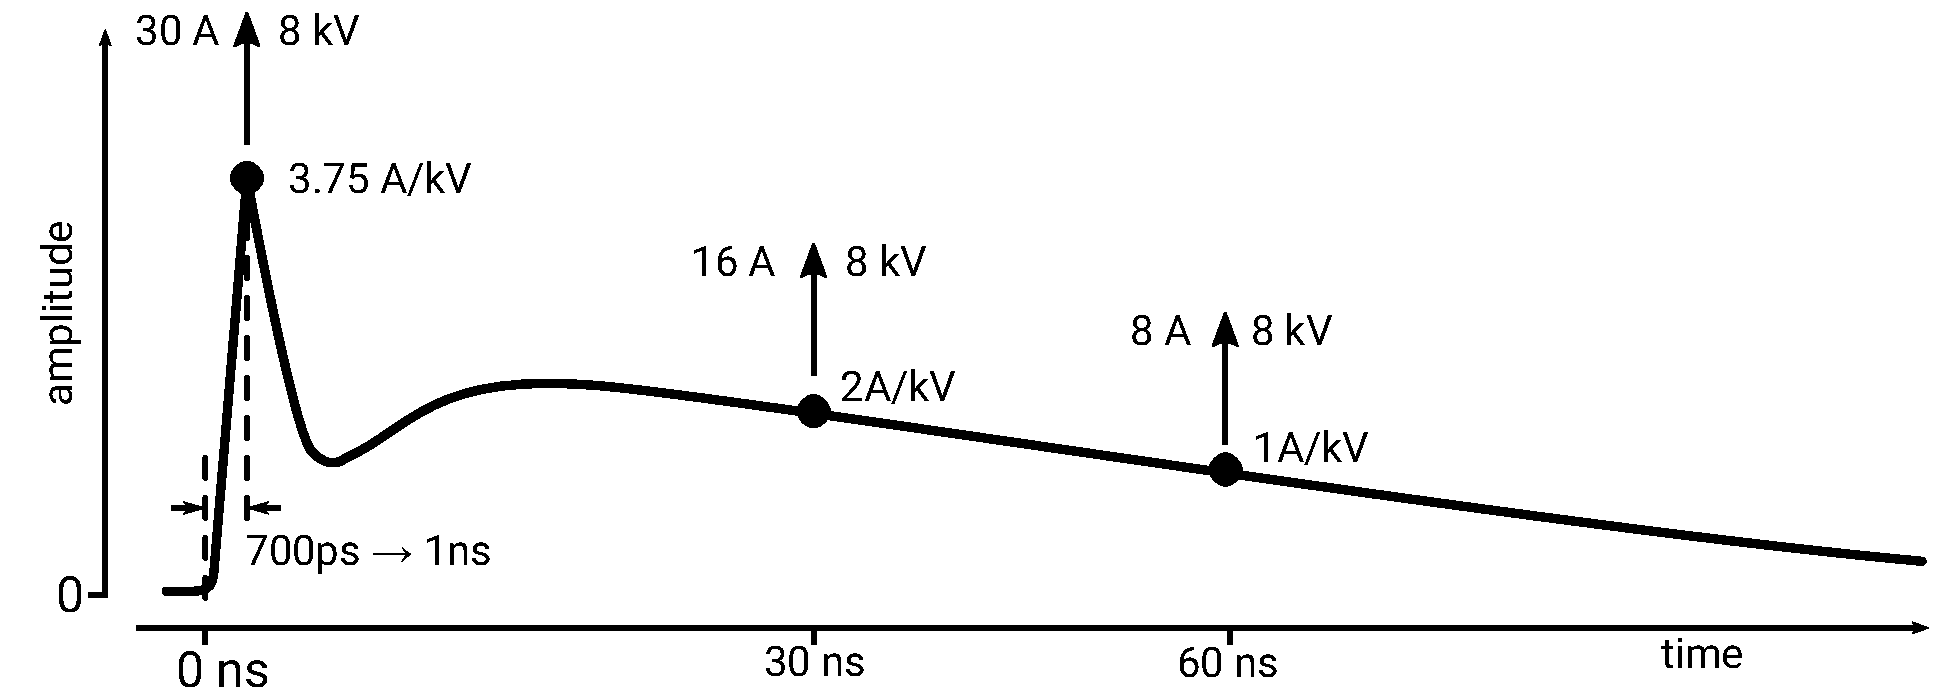
\includegraphics[width=\textwidth]{src/1/figures/iec61000-4-2_waveform.pdf}
  \caption{Main properties of an IEC 61000-4-2 pulse on a 2\textOmega\ resistive load}
  \label{iec_pulse}
\end{figure}

Other test methods exist, such as ... Test automobile ISO, Méthode DPI standardizée

\section{Méthodes d'analyse de faiblesses fonctionnelles}

% Case 1 - NXP bandgap + substrate coupling
K. Abouda details in \cite{softfailEMCIC} a case of soft-failure on an integrated automotive regulator \gls{ic}.
The failure signature is a loss of the regulated voltage when exposed to \gls{bci} ISO11452-4 \cite{iso11452}.
The test setup is provided in Fig. \ref{}.
The product is investigated manually, by searching inside the design for coupling and propagation paths, and performing multiple simulations.
Eventually, it was proven that a residue of the disturbance was coupling through the substrate on a current mirror inside the bandgap reference.
During the disturbance, bandgap voltage was shifting from its nominal value.
After some delay, the bandgap output was reaching an undervoltage threshold, causing the entire system to restart.
To avoid it, a design fix was proposed by filtering at the appropriate spot inside the design to avoid the amplification of the disturbance.

\begin{figure}[!h]
  \centering
  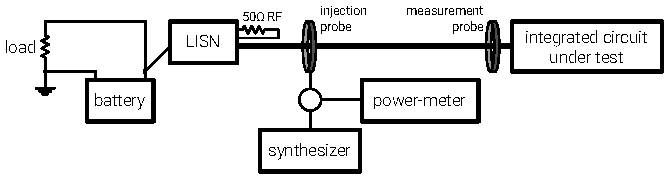
\includegraphics[width=\textwidth]{src/1/figures/bci_setup.pdf}
  \caption{Bulk Current Injection setup}
  \label{fig:bci-setup}
\end{figure}

% Case 2 - CESAME IC - paper Vrignon + Ben dhia
N. Lacrampe presents another failure case in \cite{LacrampeTransientImmunity}.
Very-fast \gls{tlp} is injected on an 0.18 \textmu{}m CMOS technology (1.8 V supply voltage) testchip.
The chip contains 6 instances on the same logic core, differing only by their power-rails architecture.
The injection on power rails is performed using a \gls{dc} block 1 nF capacitor, similarly to the \gls{dpi} standard \cite{iec62132-4}.
% What is the failure signature
An output signal of the logic core is monitored.
The susceptibility criteria is the amplitude crossing a 20\% threshold from the established logic level.
Above this threshold, the core is supposed to no longer work reliably.
It is proven that modelling the output buffer of the core logic is enough for reproducing with less than 20\% error the waveform on the output.
It is less accurate than a full-netlist simulation, but faster to simulate.
VHDL-AMS and \gls{spice} modelling are performed in this analysis.

%TODO: Pictures
% Case 3 - failures on an SDRAM
%TODO: Read reference articles in this article
In \cite{SDRAMCase}, soft-failures are studied on a SDRAM memory in operation.
The injection setup consists of a modified compact \gls{tem} cell \ref{fig:modified-tem-cell} with a reduced septum height.
Reduced dimensions result in increased field strenghts, to reach levels normally produced by an \gls{esd} gun.
The discharge waveform, injected inside the cell, is generated by a filtered \gls{tlp} and is similar in shape to IEC 61000-4-2 \cite{iec61000-4-2}.
The SDRAM chip is mounted on a board.
Data is written and read on the memory by \gls{fpga}.
Differences between incoming and outgoing data signifies a functional failure of the memory.
Only the memory is exposed to the disturbance, the rest of the board's devices are located outside of the \gls{tem} cell, on the other side of the board.
The main defect of this method is to only provide a global failure level.
It does not allow to identify which particular net or pin is the most sensitive to disturbances.

\begin{figure}[!h]
  \centering
  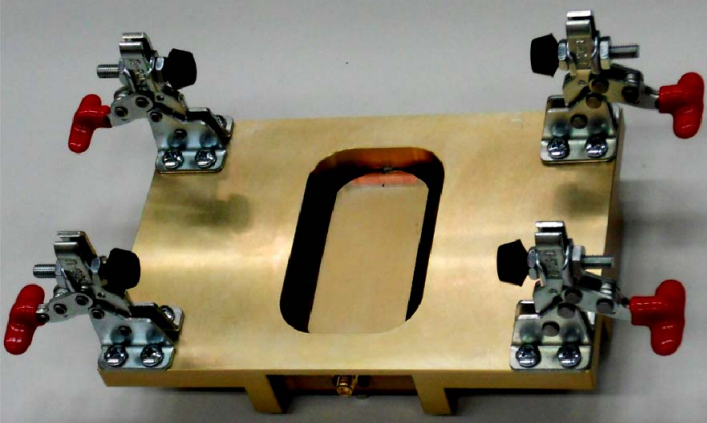
\includegraphics[width=0.6\textwidth]{src/1/figures/modified_tem_cell.png}
  \caption{Modified TEM cell from \cite{SDRAMCase}}
  \label{fig:modified-tem-cell}
\end{figure}

B. Orr reports in \cite{softFailSubsystem} errors caused by electrostatic discharges on two different camera communication buses.
Events of different severities are observed, depending on the discharge parameters.
It is attempted to determine whether the sensor or the application processor is causing the error.
The magnetic emission map is recorded with a near-field magnetic scanner to try to observe local variations in the emission spectrum because of the degradation of functionnality.
It was envisionned that soft-failure can induce significant variations in the emission spectrum of a disturbed component, and thus those variations could help localize them.
In this particular case, the root cause of failures could not be determined.

An LCD display is studied in \cite{softFailLCD}.
The device is tested with an IEC 61000-4-2 \cite{iec61000-4-2} generator, and non-destrutive problems are observed due to the discharge.
Electromagnetic disturbances cause stripes to appear on the display, optical parameters changes and blacklighting malfunctions.
System-level testing waveforms were found too complex for identifying the root cause.
A near-field injection is performed to identify which trace of the LCD's flex connector claims the lowest immunity.
The lack of resolution of the near-field probe caused multiple traces to be disturbed at once, preventing this second approach to work.
Finally, the individual track stressing was repeated with a capacitively-coupled \gls{tlp} on each individual metal track.
However, results were once more unconclusive and no metal trace could categorically be identified as more sensitive than the others.
The conclusion for this paper is that silicon level soft-error models are required for standard investigation.

An investigation method is presented in \cite{softFailMobile} to search for discharge propagation paths responsible for soft-failures on a mobile phone.
The IEC 61000-4-2 standard is chosen as testing waveform.
Metallic parts are assumed to be the main propagation paths.
To confirm this hypothesis, time-domain electromagnetic field 3D simulations of almost the entire phone are ran (see Fig. \ref{fig:mobile-phone-3d-em})
After the failure location was determined, RC-networks are used as countermeasures to protect physical inputs and outputs, like buttons, LCD inputs and connectors.

\begin{figure}[!h]
  \centering
  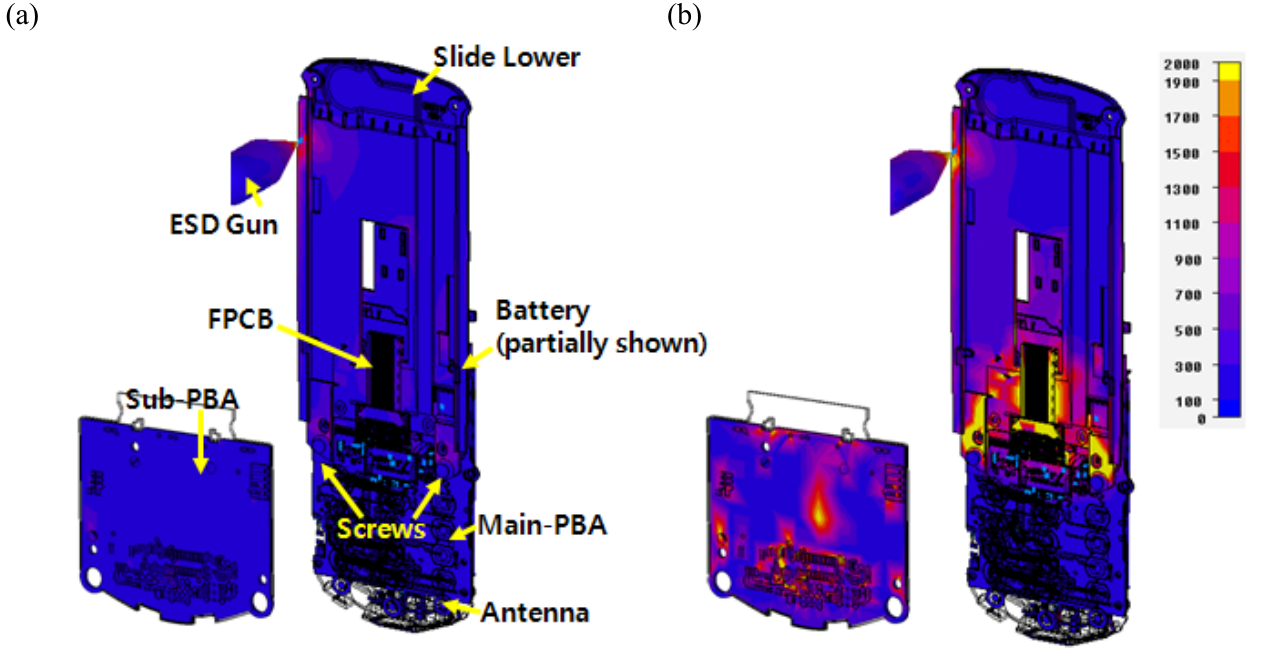
\includegraphics[width=0.8\textwidth]{src/1/figures/current_distribution_mobile.png}
  \caption{ESD Current Distribution on Mobile Phone and Backside sub-battery pack at (a) 1.0 ns and (b) 1.8 ns (Credit: \cite{softFailMobile})}
  \label{fig:mobile-phone-3d-em}
\end{figure}


Near-field scan

% Introduce near-field scanner
Electromagnetic near-field scanner measure maps of electric and magnetic field.
An electric or magnetic probe is swept closely above a device to record the emitted field in near-field conditions.
Measurements may be carried out in the frequency domain or in the time domain.
This tool was initially intended for architectural analysis such as floor-planning and power distribution analysis.
For ESD, spatial information provided by the recorded map is very useful to locate failures and malfunctions.
A comprehensive and detailed analysis of near-field antennas is done by A.D. Yaghjian in \cite{nfsFirstStudy}.
More recent work details the principle of operation, data processing and hardware requirements in \cite{near-field-scan, planarNFSAntenna, NFSMeasurements, NFScanner}.
Finally, measurement of electromagnetic emissions with surface scan method is standardized in IEC TS 61967-3 \cite{iec61967}.
The architecture of a near-field scanner is given in Fig. \ref{fig:near-field-scanner}.

\begin{figure}[!h]
  \centering
  \includegraphics[width=0.4\textwidth]{src/1/figures/architecture_near_field_scanner.pdf}
  \caption{Architecture of a near-field scanning testbench}
  \label{fig:near-field-scanner}
\end{figure}

\begin{figure}[!h]
  \centering
  \includegraphics[width=0.4\textwidth]{src/1/figures/near_field_scanner_susceptibility_map.pdf}
  \caption{Susceptibility map of a board recorded with surface scan in injection configuration \cite{}}
  \label{fig:near-field-scan-map}
\end{figure}

Revue des méthodes de modélisation

In the litterature, various ESD modelling methods can be found.
They comprise a wide range of techniques such as 3D electromagnetic and semiconductor physics simulations, compact, behavioral, physically-based and non-linear modelling.
The methods described hereafter could be used for soft-failure investigation.

M. Scholz details a mixed-mode ESD simulation approach in \cite{mixedModeESDSims}.
It is a combination of \gls{spice} and \gls{tcad} models, simulated in \gls{spice} environment.
The author indicates that the combination of physical device models and standard simulations provides higher accuracy and more realistic simulations than behavioral \gls{spice} models.
Using this complex simulation tool, on-chip and off-chip device interactions are studied, in powered and unpowered conditions.

In \cite{usb2ESDProtection}, TLP characterizations serves as an I(V) model for both external protections and an \gls{ic} pin.
The \gls{pcb} S-parameters are extracted from the board layout, using Momentum software (Agilent Technology).
It is electrically model with lumped R,L,C,G elements.
The modelling approach proved successful for simulation interactions between external devices and on-chip structures.
This method is interesting for soft-failure analysis because it is thorough and complete and enables accurate ESD simulation.

% IBIS is not enough for modelling an IC pin for ESD simulations
The Input Output Buffer Information Specification (IBIS) \cite{ibis-spec} is a behavioral, black-box model for performing signal integrity simulation on digital circuits.
It is widespread in the digital \gls{asic} world because it enables accurate simulations without disclosing circuit or process information.
It was envisionned that IBIS models could also be used or extended for ESD.
It is demonstrated in \cite{ibisImprovementFabrice} that the model lacks some parameters for EMC and ESD simulations.
It comprises a current versus voltage characteristic of \gls{io}s, similar to what can be extracted by a TLP, however the IBIS model is not defined for fast impulses and high injection.

N. Lacrampe proposes in \cite{LacrampeTransientImmunity} to perform 3D electromagnetic simulations at silicon level, using the integrated circuit layout, to deduce the amount of capacitive couplings between Vdd and Vss rails.
The extraction is performed with HFSS software (Ansoft).
The goal of this analysis is to predict the susceptibility of integrated circuits against electrostatic discharges.
\gls{pcb} tracks are modeled by a distributed RLC network.
The package data from the IBIS model \cite{ibis-spec} was used in the simulations.
Finally, a TLP stress generator is modelled using a lookup table I(V) component, in series with a 50\textOmega{} resistor.

Once again, electromagnetic fullwave simulations are conducted in powered-on ESD analysis in \cite{softFailMobile}.
System-level components are simulated, such as PCB, metallic casing and battery back.
3D EM simulations helps to identify the main discharge paths and locate the failure.
